\documentclass[color=usenames,dvipsnames]{beamer}\usepackage[]{graphicx}\usepackage[]{color}
%% maxwidth is the original width if it is less than linewidth
%% otherwise use linewidth (to make sure the graphics do not exceed the margin)
\makeatletter
\def\maxwidth{ %
  \ifdim\Gin@nat@width>\linewidth
    \linewidth
  \else
    \Gin@nat@width
  \fi
}
\makeatother

\definecolor{fgcolor}{rgb}{0, 0, 0}
\newcommand{\hlnum}[1]{\textcolor[rgb]{0.69,0.494,0}{#1}}%
\newcommand{\hlstr}[1]{\textcolor[rgb]{0.749,0.012,0.012}{#1}}%
\newcommand{\hlcom}[1]{\textcolor[rgb]{0.514,0.506,0.514}{\textit{#1}}}%
\newcommand{\hlopt}[1]{\textcolor[rgb]{0,0,0}{#1}}%
\newcommand{\hlstd}[1]{\textcolor[rgb]{0,0,0}{#1}}%
\newcommand{\hlkwa}[1]{\textcolor[rgb]{0,0,0}{\textbf{#1}}}%
\newcommand{\hlkwb}[1]{\textcolor[rgb]{0,0.341,0.682}{#1}}%
\newcommand{\hlkwc}[1]{\textcolor[rgb]{0,0,0}{\textbf{#1}}}%
\newcommand{\hlkwd}[1]{\textcolor[rgb]{0.004,0.004,0.506}{#1}}%
\let\hlipl\hlkwb

\usepackage{framed}
\makeatletter
\newenvironment{kframe}{%
 \def\at@end@of@kframe{}%
 \ifinner\ifhmode%
  \def\at@end@of@kframe{\end{minipage}}%
  \begin{minipage}{\columnwidth}%
 \fi\fi%
 \def\FrameCommand##1{\hskip\@totalleftmargin \hskip-\fboxsep
 \colorbox{shadecolor}{##1}\hskip-\fboxsep
     % There is no \\@totalrightmargin, so:
     \hskip-\linewidth \hskip-\@totalleftmargin \hskip\columnwidth}%
 \MakeFramed {\advance\hsize-\width
   \@totalleftmargin\z@ \linewidth\hsize
   \@setminipage}}%
 {\par\unskip\endMakeFramed%
 \at@end@of@kframe}
\makeatother

\definecolor{shadecolor}{rgb}{.97, .97, .97}
\definecolor{messagecolor}{rgb}{0, 0, 0}
\definecolor{warningcolor}{rgb}{1, 0, 1}
\definecolor{errorcolor}{rgb}{1, 0, 0}
\newenvironment{knitrout}{}{} % an empty environment to be redefined in TeX

\usepackage{alltt}
%\documentclass[color=usenames,dvipsnames,handout]{beamer}




\usepackage[sans]{../../lab1}
\usepackage{bm}


\hypersetup{pdftex,pdfstartview=FitV}









%% New command for inline code that isn't to be evaluated
\definecolor{inlinecolor}{rgb}{0.878, 0.918, 0.933}
\newcommand{\inr}[1]{\colorbox{inlinecolor}{\texttt{#1}}}
\IfFileExists{upquote.sty}{\usepackage{upquote}}{}
\begin{document}




\begin{frame}[plain]
  \huge
  \begin{center}
    {\color{PineGreen}{Generalized Linear Models (GLMs)}} \\
    \vfill
    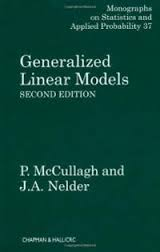
\includegraphics[width=0.3\textwidth]{McCullagh-Nelder} \\
    \large \vfill
    November 13 \& 15, 2017
  \end{center}
%  \note{not to be confused with General Linear Model}
\end{frame}



\section{Generalized linear models}

\begin{frame}
  \frametitle{Motivation}
  %% {\bf Limitations of linear models}
  %% \begin{itemize}[<+->]
  %%   \item Not appropriate when response variable is discrete
  %%     (e.g. binary)
  %%   \item Sometimes transformations can't make residuals normal
  %%   \item Predictions might not be on the correct scale
  %%   \item Constant variance assumption can be problematic
  %% \end{itemize}
  \large
  \uncover<1->{{\bf Benefits of generalized linear models}}
  \begin{itemize}%[<+->]
    \item<2-> The residuals don't have to be normally distributed
    \item<3-> The response variable can be binary, integer,
      strictly-positive, etc...
    \item<4-> The variance is not assumed to be constant
    \item<5-> Useful for manipulative experiments or observational
      studies, just like linear models.
  \end{itemize}
  \vfill
  \uncover<6->{
  {\bf Examples}
  \begin{itemize}
    \item Presence-absence studies
    \item Studies of survival
    \item Seed germination studies
    \item Analysis of zero-inflated count data
  \end{itemize}
  }
\end{frame}




% \begin{frame}
%   \frametitle{From linear to generalized linear}
% \only<1>{
%   {\bf A linear model is an equation of the form:}
%   \[
%     \mu_i = \beta_0 + \beta_1 x1_i + \beta_2 x2_i + \ldots + \beta_p xp_i
%   \]
%   }
% \only<2>{
%   {\bf A generalized linear model is an equation of the form:}
%   \[
%     g(\eta_i) = \beta_0 + \beta_1 x1_i + \beta_2 x2_i + \ldots + \beta_p xp_i
%   \]
%   }
% \end{frame}


\begin{frame}
  \frametitle{From linear to generalized linear}
%  {\bf Linear model}
%  \begin{gather*}
%    \mu_i = \beta_0 + \beta_1 x_{i1} + \beta_2 x_{i2} + \cdots \\
%    y_i \sim \mathrm{Normal}(\mu_i, \sigma^2)
%  \end{gather*}
%  \pause
  {\bf Generalized Linear model}
  \begin{gather*}
    g(\mu_i) = \beta_0 + \beta_1 x_{i1} + \beta_2 x_{i2} + \cdots \\
    y_i \sim f(\mu_i)
  \end{gather*}
  \pause
  {\bf where} \\
  $g$ is a link function, such as the log or logit link \\
  \pause
  $f$ is a probability distribution such as the binomial or Poisson
%  that determines (usually) the variance %(there is no $\sigma^2$ parameter!)
\end{frame}


\begin{frame}
  \frametitle{Alternative representations}
  {\bf This:}
  \begin{gather*}
    g(\mu_i) = \beta_0 + \beta_1 x_{i1} + \beta_2 x_{i2} + \cdots \\
    y_i \sim f(\mu_i)
  \end{gather*}
  \pause
  {\bf Is the same as this:}
  \begin{gather*}
    \mu_i = g^{-1}(\beta_0 + \beta_1 x_{i1} + \beta_2 x_{i2} + \cdots) \\
    y_i \sim f(\mu_i)
  \end{gather*}
  \pause
  {\bf Is the same as this:}
  \begin{gather*}
    g(\mu_i) = {\bf X}{\bm \beta} \\
    y_i \sim f(\mu_i)
  \end{gather*}
\end{frame}


\begin{frame}
  \frametitle{Link functions}
%  \begin{itemize}[<+->]
%    \item
  An inverse link function ($g^{-1}$) transforms values from the $(-\infty,\infty)$
  scale to the scale of interest, such as $(0,1)$ for probabilities  \\
  \pause
  \vfill
%    \item
  The link function ($g$) does the reverse \\
%    \item
  \pause
  \vfill
  The two link functions that you will see most often are the
      ``logit'' and ``log'' links.
%  \end{itemize}
\end{frame}


\begin{frame}
  \frametitle{Link functions}
  \begin{tabular}{llcc}
    \hline
    Distribution & link name\footnote{These are the most commonly used link functions for each distribution, but others are available} & link equation             & inverse link equation       \\
    \hline
%    Normal       & identity  & $\mu$                     & ${\bf X}{\bm \beta}$  \\
%                 &           &                           &                             \\
    Binomial     & logit     & $\log(\frac{p}{1-p})$ & $\frac{\exp({\bf
          X}{\bm \beta})}{1 + \exp({\bf X}{\bm \beta})}$                        \\
                 &           &                           &                             \\
    Poisson      & log       & $\log(\lambda)$               & $\exp({\bf X}{\bm \beta})$  \\
    \hline
  \end{tabular}

\pause
\vfill

\begin{tabular}{llcc}
    \hline
    Distribution & link name & link in {\bf R}  & inv link in {\bf R}       \\
    \hline
    Binomial     & logit     & {\tt qlogis} & {\tt plogis}                        \\
                 &           &                           &                             \\
    Poisson      & log       & {\tt log}    & {\tt exp}  \\
    \hline
  \end{tabular}
\end{frame}






%% \begin{frame}[fragile]
%%   \frametitle{Log link example}
%% <<>>=
%% beta0 <- 5
%% beta1 <- -0.08
%% elevation <- 100
%% eta <- beta0 + beta1*elevation
%% eta
%% @
%% \pause
%% {\bf How do we convert -3 to a positive value? \par}
%% \pause
%% {\bf Use the inverse-log function, i.e. the exponential function:}
%% <<>>=
%% exp(-3)
%% @
%% \end{frame}






\begin{frame}[fragile]
  \frametitle{Logit link example}
  \vspace{-5pt}
  \scriptsize
\begin{knitrout}\scriptsize
\definecolor{shadecolor}{rgb}{0.878, 0.918, 0.933}\color{fgcolor}\begin{kframe}
\begin{alltt}
\hlstd{beta0} \hlkwb{<-} \hlnum{5}
\hlstd{beta1} \hlkwb{<-} \hlopt{-}\hlnum{0.08}
\hlstd{elevation} \hlkwb{<-} \hlnum{100}
\hlstd{(logit.p} \hlkwb{<-} \hlstd{beta0} \hlopt{+} \hlstd{beta1}\hlopt{*}\hlstd{elevation)}
\end{alltt}
\begin{verbatim}
## [1] -3
\end{verbatim}
\end{kframe}
\end{knitrout}
\pause
{How do we convert -3 to a probability? \pause Use the
  inverse-link: \\}
\begin{knitrout}\scriptsize
\definecolor{shadecolor}{rgb}{0.878, 0.918, 0.933}\color{fgcolor}\begin{kframe}
\begin{alltt}
\hlstd{p} \hlkwb{<-} \hlkwd{exp}\hlstd{(logit.p)}\hlopt{/}\hlstd{(}\hlnum{1}\hlopt{+}\hlkwd{exp}\hlstd{(logit.p))}
\hlstd{p}
\end{alltt}
\begin{verbatim}
## [1] 0.04742587
\end{verbatim}
\end{kframe}
\end{knitrout}
\pause
{Same as:}
\begin{knitrout}\scriptsize
\definecolor{shadecolor}{rgb}{0.878, 0.918, 0.933}\color{fgcolor}\begin{kframe}
\begin{alltt}
\hlkwd{plogis}\hlstd{(logit.p)}
\end{alltt}
\begin{verbatim}
## [1] 0.04742587
\end{verbatim}
\end{kframe}
\end{knitrout}
\pause
{To go back, use the link function itself:}
\begin{knitrout}\scriptsize
\definecolor{shadecolor}{rgb}{0.878, 0.918, 0.933}\color{fgcolor}\begin{kframe}
\begin{alltt}
\hlkwd{log}\hlstd{(p}\hlopt{/}\hlstd{(}\hlnum{1}\hlopt{-}\hlstd{p))}
\end{alltt}
\begin{verbatim}
## [1] -3
\end{verbatim}
\begin{alltt}
\hlkwd{qlogis}\hlstd{(p)}
\end{alltt}
\begin{verbatim}
## [1] -3
\end{verbatim}
\end{kframe}
\end{knitrout}
\end{frame}



\begin{frame}[fragile]
  \frametitle{Logit link example}
\begin{knitrout}\scriptsize
\definecolor{shadecolor}{rgb}{0.878, 0.918, 0.933}\color{fgcolor}\begin{kframe}
\begin{alltt}
\hlkwd{plot}\hlstd{(}\hlkwa{function}\hlstd{(}\hlkwc{x}\hlstd{)} \hlnum{5} \hlopt{+ -}\hlnum{0.08}\hlopt{*}\hlstd{x,} \hlkwc{from}\hlstd{=}\hlnum{0}\hlstd{,} \hlkwc{to}\hlstd{=}\hlnum{100}\hlstd{,}
     \hlkwc{main}\hlstd{=}\hlstr{"Without the logit transformation"}\hlstd{,}
     \hlkwc{xlab}\hlstd{=}\hlstr{"Elevation"}\hlstd{,} \hlkwc{ylab}\hlstd{=}\hlstr{"logit(prob of occurrence)"}\hlstd{)}
\end{alltt}
\end{kframe}
\end{knitrout}
%\begin{center}
\centering
  \includegraphics[width=\textwidth]{figure/nologit-1} \\
%\end{center}
\end{frame}




\begin{frame}[fragile]
  \frametitle{Logit link example}
\begin{knitrout}\scriptsize
\definecolor{shadecolor}{rgb}{0.878, 0.918, 0.933}\color{fgcolor}\begin{kframe}
\begin{alltt}
\hlkwd{plot}\hlstd{(}\hlkwa{function}\hlstd{(}\hlkwc{x}\hlstd{)} \hlkwd{plogis}\hlstd{(}\hlnum{5} \hlopt{+ -}\hlnum{0.08}\hlopt{*}\hlstd{x),} \hlkwc{from}\hlstd{=}\hlnum{0}\hlstd{,} \hlkwc{to}\hlstd{=}\hlnum{100}\hlstd{,}
     \hlkwc{main}\hlstd{=}\hlstr{"With the logit transformation"}\hlstd{,}
     \hlkwc{xlab}\hlstd{=}\hlstr{"Elevation"}\hlstd{,} \hlkwc{ylab}\hlstd{=}\hlstr{"Probability of occurrence"}\hlstd{)}
\end{alltt}
\end{kframe}
\end{knitrout}
%\begin{center}
\centering
  \includegraphics[width=\textwidth]{figure/logit2-1} \\
%\end{center}
\end{frame}





\section{Logistic regression}


\begin{frame}
  \frametitle{Logistic Regression}
%  \begin{itemize}%[<+->]
%    \item<1->
  Logistic regression is a specific type of GLM in which the
      response variable follows a binomial distribution and the link
      function is the logit \\
  \pause
  \vfill
%    \item<2->
  It would be better to call it ``binomial regression'' since other
      link functions (e.g. the probit) can be used \\
%    \item<3->
  \pause
  \vfill
  Appropriate when the response is binary or a count with an
  upper limit
%    \item<4->
  \pause
  \vfill
  {\bf Examples:}
      \begin{itemize}
        \normalsize
        \item Presence/absence studies
        \item Survival studies
        \item Disease prevalance studies
      \end{itemize}
%  \end{itemize}
\end{frame}


\begin{frame}
  \frametitle{Logistic Regression}
    \begin{gather*}
      \mathrm{logit}(p_i) = \beta_0 + \beta_1 x_{i1} + \beta_2 x_{i2} + \cdots \\
      y_i \sim \mathrm{Binomial}(N, p_i)
  \end{gather*}
  \pause
  {\bf where: \\}
  $N$ is the number of ``trials'' (e.g. coin flips) \\
  $p_i$ is the probability of a success for sample unit $i$
\end{frame}



\begin{frame}[fragile]
  \frametitle{Binomial distribution}% - fair coin}
  \vspace{-0.4cm}
  \note{Have students flip coins}
\begin{center}
\begin{knitrout}
\definecolor{shadecolor}{rgb}{0.878, 0.918, 0.933}\color{fgcolor}
\includegraphics[width=0.9\textwidth]{figure/binom1-1} 

\end{knitrout}
\end{center}
\vfill
\end{frame}



\begin{frame}[fragile]
  \frametitle{Binomial distribution}% - warped coin}
  \vspace{-0.4cm}
\begin{center}
\begin{knitrout}
\definecolor{shadecolor}{rgb}{0.878, 0.918, 0.933}\color{fgcolor}
\includegraphics[width=0.9\textwidth]{figure/binom2-1} 

\end{knitrout}
\end{center}
\end{frame}




\begin{frame}
  \frametitle{Binomial Distribution}
  {\bf Properties}
  \begin{itemize}
    \item The mean is $Np$
    \item The variance is $Np(1-p)$
  \end{itemize}
  \pause
  \vfill
  {\bf Bernoulli distribution}
  \begin{itemize}
    \item The Bernoulli distribution is a binomial distribution with a
      single trial ($N=1$)
%    \item Think of it as a single coin flip
    \item Logistic regression is usually done in this context, such
      that the response variable is 0/1 or No/Yes or Bad/Good, etc$\dots$
  \end{itemize}
\end{frame}


\section{The {\tt glm} function}

\begin{frame}[fragile]
  \frametitle{Worked example using {\tt glm}}

\begin{columns}
  \begin{column}{0.45\textwidth}
    \tiny
\begin{knitrout}\tiny
\definecolor{shadecolor}{rgb}{0.878, 0.918, 0.933}\color{fgcolor}\begin{kframe}
\begin{alltt}
\hlstd{frogData}
\end{alltt}
\begin{verbatim}
##    presence abundance elevation habitat
## 1         0         0        58     Oak
## 2         0         3       191     Oak
## 3         0         0        43     Oak
## 4         1        15       374     Oak
## 5         1         7       337     Oak
## 6         0         0        64     Oak
## 7         1         1       195     Oak
## 8         0         1       263     Oak
## 9         1         3       181     Oak
## 10        1         3        59     Oak
## 11        1        60       489   Maple
## 12        1         9       317   Maple
## 13        0         0        12   Maple
## 14        1         4       245   Maple
## 15        1        38       474   Maple
## 16        0         0        83   Maple
## 17        1        42       467   Maple
## 18        1        52       485   Maple
## 19        1        12       335   Maple
## 20        1         1        20   Maple
## 21        1        31       430    Pine
## 22        0         1       223    Pine
## 23        0         0        68    Pine
## 24        1        47       483    Pine
## 25        1         0        78    Pine
## 26        1         4       214    Pine
## 27        0         1        64    Pine
## 28        0         2        73    Pine
## 29        1         3       162    Pine
## 30        1        40       468    Pine
\end{verbatim}
\end{kframe}
\end{knitrout}
  \end{column}
  \begin{column}{0.54\textwidth}
    \minipage[c][0.7\textheight][s]{\columnwidth}
    \small
    First we will model the presence-absence response variable to
    determine if elevation and habitat affect the probability of
    occurrence. \par
    \pause
    \vspace{1cm}
    Then we will model abundance.
    \endminipage
  \end{column}
\end{columns}
\end{frame}



\begin{frame}[fragile]
  \frametitle{Raw data}
  \tiny
%  \vspace{-0.5cm}
%\begin{center}
\begin{knitrout}\tiny
\definecolor{shadecolor}{rgb}{0.878, 0.918, 0.933}\color{fgcolor}\begin{kframe}
\begin{alltt}
\hlkwd{plot}\hlstd{(presence} \hlopt{~} \hlstd{elevation, frogData,}
     \hlkwc{xlab}\hlstd{=}\hlstr{"Elevation"}\hlstd{,} \hlkwc{ylab}\hlstd{=}\hlstr{"Frog Occurrence"}\hlstd{)}
\end{alltt}
\end{kframe}
\end{knitrout}
\centering
  \includegraphics[width=0.7\textwidth]{figure/raw-elev-1} \\
%\end{center}
\end{frame}




\begin{frame}[fragile]
  \frametitle{Raw data}
%  \tiny
\begin{center}
\begin{knitrout}\tiny
\definecolor{shadecolor}{rgb}{0.878, 0.918, 0.933}\color{fgcolor}\begin{kframe}
\begin{alltt}
\hlstd{group.prop} \hlkwb{<-} \hlkwd{tapply}\hlstd{(frogData}\hlopt{$}\hlstd{presence, frogData}\hlopt{$}\hlstd{habitat, mean)}
\hlkwd{barplot}\hlstd{(group.prop,} \hlkwc{ylab}\hlstd{=}\hlstr{"Proportion of sites with frogs"}\hlstd{)}
\end{alltt}
\end{kframe}
\end{knitrout}
  \includegraphics[width=0.7\textwidth]{figure/raw-habitat-1}
\end{center}
%\vspace{0.5cm}
\end{frame}





\begin{frame}[fragile]
  \frametitle{The function {\tt glm}}
  \footnotesize
\begin{knitrout}\tiny
\definecolor{shadecolor}{rgb}{0.878, 0.918, 0.933}\color{fgcolor}\begin{kframe}
\begin{alltt}
\hlstd{fm1} \hlkwb{<-} \hlkwd{glm}\hlstd{(presence} \hlopt{~} \hlstd{habitat} \hlopt{+} \hlstd{elevation,}
           \hlkwc{family}\hlstd{=}\hlkwd{binomial}\hlstd{(}\hlkwc{link}\hlstd{=}\hlstr{"logit"}\hlstd{),} \hlkwc{data}\hlstd{=frogData)}
\end{alltt}
\end{kframe}
\end{knitrout}
\pause
\begin{knitrout}\tiny
\definecolor{shadecolor}{rgb}{0.878, 0.918, 0.933}\color{fgcolor}\begin{kframe}
\begin{alltt}
\hlkwd{summary}\hlstd{(fm1)}
\end{alltt}
\begin{verbatim}
## 
## Call:
## glm(formula = presence ~ habitat + elevation, family = binomial(link = "logit"), 
##     data = frogData)
## 
## Deviance Residuals: 
##     Min       1Q   Median       3Q      Max  
## -1.6608  -0.7663   0.1610   0.5031   1.7773  
## 
## Coefficients:
##               Estimate Std. Error z value Pr(>|z|)  
## (Intercept)  -2.053609   1.092854  -1.879   0.0602 .
## habitatMaple  1.220668   1.324680   0.921   0.3568  
## habitatPine   0.281932   1.107228   0.255   0.7990  
## elevation     0.011950   0.004774   2.503   0.0123 *
## ---
## Signif. codes:  0 '***' 0.001 '**' 0.01 '*' 0.05 '.' 0.1 ' ' 1
## 
## (Dispersion parameter for binomial family taken to be 1)
## 
##     Null deviance: 39.429  on 29  degrees of freedom
## Residual deviance: 25.577  on 26  degrees of freedom
## AIC: 33.577
## 
## Number of Fisher Scoring iterations: 6
\end{verbatim}
\end{kframe}
\end{knitrout}
\end{frame}


%% \begin{frame}[fragile]
%%   \frametitle{Test main effects}
%%   \footnotesize
%% <<>>=
%% anova(fm1, test="Chisq")
%% @
%% \end{frame}


\begin{frame}[fragile]
  \frametitle{Occurrence probability and elevation}
  \footnotesize
\begin{knitrout}
\definecolor{shadecolor}{rgb}{0.878, 0.918, 0.933}\color{fgcolor}\begin{kframe}
\begin{alltt}
\hlstd{newdat} \hlkwb{<-} \hlkwd{data.frame}\hlstd{(}\hlkwc{elevation}\hlstd{=}\hlkwd{seq}\hlstd{(}\hlnum{12}\hlstd{,} \hlnum{489}\hlstd{,} \hlkwc{length}\hlstd{=}\hlnum{50}\hlstd{),}
                     \hlkwc{habitat}\hlstd{=}\hlstr{"Oak"}\hlstd{)}
\hlkwd{head}\hlstd{(newdat)}
\end{alltt}
\begin{verbatim}
##   elevation habitat
## 1  12.00000     Oak
## 2  21.73469     Oak
## 3  31.46939     Oak
## 4  41.20408     Oak
## 5  50.93878     Oak
## 6  60.67347     Oak
\end{verbatim}
\end{kframe}
\end{knitrout}
\pause
{\bf To get confidence intervals on (0,1) scale, predict on linear
  (link) scale and then backtransform using inverse-link}
\pause
%\scriptsize
\begin{knitrout}\footnotesize
\definecolor{shadecolor}{rgb}{0.878, 0.918, 0.933}\color{fgcolor}\begin{kframe}
\begin{alltt}
\hlstd{pred.link} \hlkwb{<-} \hlkwd{predict}\hlstd{(fm1,} \hlkwc{newdata}\hlstd{=newdat,} \hlkwc{se.fit}\hlstd{=}\hlnum{TRUE}\hlstd{,} \hlkwc{type}\hlstd{=}\hlstr{"link"}\hlstd{)}
\hlstd{newdat}\hlopt{$}\hlstd{mu} \hlkwb{<-} \hlkwd{plogis}\hlstd{(pred.link}\hlopt{$}\hlstd{fit)}
\hlstd{newdat}\hlopt{$}\hlstd{lower} \hlkwb{<-} \hlkwd{plogis}\hlstd{(pred.link}\hlopt{$}\hlstd{fit} \hlopt{-} \hlnum{1.96}\hlopt{*}\hlstd{pred.link}\hlopt{$}\hlstd{se.fit)}
\hlstd{newdat}\hlopt{$}\hlstd{upper} \hlkwb{<-} \hlkwd{plogis}\hlstd{(pred.link}\hlopt{$}\hlstd{fit} \hlopt{+} \hlnum{1.96}\hlopt{*}\hlstd{pred.link}\hlopt{$}\hlstd{se.fit)}
\end{alltt}
\end{kframe}
\end{knitrout}
\end{frame}



\begin{frame}[fragile]
  \frametitle{Occurrence probability and elevation}
  \tiny
\begin{knitrout}\tiny
\definecolor{shadecolor}{rgb}{0.878, 0.918, 0.933}\color{fgcolor}
\includegraphics[width=\maxwidth]{figure/pred1-1} 

\end{knitrout}
%  \begin{center}
\centering
    \includegraphics[width=0.85\textwidth]{figure/pred1-1} \\
%  \end{center}
\end{frame}







\section{Poisson regression}



\begin{frame}
  \frametitle{Poisson Regression}
  \Large
    \begin{gather*}
      \mathrm{log}(\lambda_i) = \beta_0 + \beta_1 x_{i1} + \beta_2 x_{i2} + \cdots \\
      y_i \sim \mathrm{Poisson}(\lambda_i)
  \end{gather*}
  \pause
  {\bf where: \\}
  $\lambda_i$ is the expected value of $y_i$ \\
\end{frame}



\begin{frame}
  \frametitle{Poisson regression}
  \large
  {\bf Useful for:}
  \begin{itemize}
    \item Count data
    \item Number of events in time intervals
    \item Other types of integer data
  \end{itemize}
  \pause
  \vfill
  {\bf Properties}
  \begin{itemize}
    \item The mean ($\lambda$) is equal to the variance
    \item This is an assumption of the Poisson model
    \item Like all assumptions, it can be relaxed if you have enough data
  \end{itemize}
\end{frame}




\begin{frame}[fragile]
  \frametitle{Poisson distribution}



\begin{center}
  \only<1>{\includegraphics[width=0.75\textwidth]{figure/pois1-1}}
  \only<2 | handout:0>{\includegraphics[width=0.75\textwidth]{figure/pois2-1}}
  \only<3 | handout:0>{\includegraphics[width=0.75\textwidth]{figure/pois3-1}}
\end{center}
\end{frame}









\begin{frame}[fragile]
  \frametitle{Log link example}
  \footnotesize
\begin{knitrout}\footnotesize
\definecolor{shadecolor}{rgb}{0.878, 0.918, 0.933}\color{fgcolor}\begin{kframe}
\begin{alltt}
\hlkwd{plot}\hlstd{(}\hlkwa{function}\hlstd{(}\hlkwc{x}\hlstd{)} \hlnum{5} \hlopt{+ -}\hlnum{0.08}\hlopt{*}\hlstd{x,} \hlkwc{from}\hlstd{=}\hlnum{0}\hlstd{,} \hlkwc{to}\hlstd{=}\hlnum{100}\hlstd{,}
     \hlkwc{main}\hlstd{=}\hlstr{"Without the log transformation"}\hlstd{,}
     \hlkwc{xlab}\hlstd{=}\hlstr{"Elevation"}\hlstd{,} \hlkwc{ylab}\hlstd{=}\hlstr{"log(Expected abundance)"}\hlstd{)}
\end{alltt}
\end{kframe}
\end{knitrout}
\begin{center}
  \includegraphics[width=\textwidth]{figure/nolog-1}
\end{center}
\end{frame}




\begin{frame}[fragile]
  \frametitle{Log link example}
  \footnotesize
\begin{knitrout}
\definecolor{shadecolor}{rgb}{0.878, 0.918, 0.933}\color{fgcolor}\begin{kframe}
\begin{alltt}
\hlkwd{plot}\hlstd{(}\hlkwa{function}\hlstd{(}\hlkwc{x}\hlstd{)} \hlkwd{exp}\hlstd{(}\hlnum{5} \hlopt{+ -}\hlnum{0.08}\hlopt{*}\hlstd{x),} \hlkwc{from}\hlstd{=}\hlnum{0}\hlstd{,} \hlkwc{to}\hlstd{=}\hlnum{100}\hlstd{,}
     \hlkwc{main}\hlstd{=}\hlstr{"With the log transformation"}\hlstd{,}
     \hlkwc{xlab}\hlstd{=}\hlstr{"Elevation"}\hlstd{,} \hlkwc{ylab}\hlstd{=}\hlstr{"Expected abundance"}\hlstd{)}
\end{alltt}
\end{kframe}
\end{knitrout}
\begin{center}
  \includegraphics[width=\textwidth]{figure/log-1}
\end{center}
\end{frame}





\begin{frame}[fragile]
  \frametitle{The function {\tt glm}}
  \footnotesize
\begin{knitrout}\tiny
\definecolor{shadecolor}{rgb}{0.878, 0.918, 0.933}\color{fgcolor}\begin{kframe}
\begin{alltt}
\hlstd{fm2} \hlkwb{<-} \hlkwd{glm}\hlstd{(abundance} \hlopt{~} \hlstd{habitat} \hlopt{+} \hlstd{elevation,}
           \hlkwc{family}\hlstd{=}\hlkwd{poisson}\hlstd{(}\hlkwc{link}\hlstd{=}\hlstr{"log"}\hlstd{),} \hlkwc{data}\hlstd{=frogData)}
\end{alltt}
\end{kframe}
\end{knitrout}
\pause
\begin{knitrout}\tiny
\definecolor{shadecolor}{rgb}{0.878, 0.918, 0.933}\color{fgcolor}\begin{kframe}
\begin{alltt}
\hlkwd{summary}\hlstd{(fm2)}
\end{alltt}
\begin{verbatim}
## 
## Call:
## glm(formula = abundance ~ habitat + elevation, family = poisson(link = "log"), 
##     data = frogData)
## 
## Deviance Residuals: 
##     Min       1Q   Median       3Q      Max  
## -1.8207  -0.9818  -0.1200   0.6251   2.3868  
## 
## Coefficients:
##               Estimate Std. Error z value Pr(>|z|)    
## (Intercept)  -1.284839   0.267329  -4.806 1.54e-06 ***
## habitatMaple  0.262192   0.215133   1.219    0.223    
## habitatPine   0.229873   0.216865   1.060    0.289    
## elevation     0.010211   0.000677  15.084  < 2e-16 ***
## ---
## Signif. codes:  0 '***' 0.001 '**' 0.01 '*' 0.05 '.' 0.1 ' ' 1
## 
## (Dispersion parameter for poisson family taken to be 1)
## 
##     Null deviance: 691.975  on 29  degrees of freedom
## Residual deviance:  28.057  on 26  degrees of freedom
## AIC: 123.21
## 
## Number of Fisher Scoring iterations: 5
\end{verbatim}
\end{kframe}
\end{knitrout}
\end{frame}


%% \begin{frame}[fragile]
%%   \frametitle{Test main effects}
%%   \footnotesize
%% <<>>=
%% anova(fm1, test="Chisq")
%% @
%% \end{frame}


\begin{frame}[fragile]
  \frametitle{Prediction}
  \footnotesize
\begin{knitrout}\footnotesize
\definecolor{shadecolor}{rgb}{0.878, 0.918, 0.933}\color{fgcolor}\begin{kframe}
\begin{alltt}
\hlstd{newdat} \hlkwb{<-} \hlkwd{data.frame}\hlstd{(}\hlkwc{elevation}\hlstd{=}\hlkwd{seq}\hlstd{(}\hlnum{12}\hlstd{,} \hlnum{489}\hlstd{,} \hlkwc{length}\hlstd{=}\hlnum{50}\hlstd{),}
                     \hlkwc{habitat}\hlstd{=}\hlstr{"Oak"}\hlstd{)}
\hlkwd{head}\hlstd{(newdat)}
\end{alltt}
\begin{verbatim}
##   elevation habitat
## 1  12.00000     Oak
## 2  21.73469     Oak
## 3  31.46939     Oak
## 4  41.20408     Oak
## 5  50.93878     Oak
## 6  60.67347     Oak
\end{verbatim}
\end{kframe}
\end{knitrout}
\pause
{\bf To get confidence intervals on (0,$\infty$) scale, predict on linear
  (link) scale and then backtransform using inverse-link}
\pause
%\scriptsize
\begin{knitrout}\scriptsize
\definecolor{shadecolor}{rgb}{0.878, 0.918, 0.933}\color{fgcolor}\begin{kframe}
\begin{alltt}
\hlstd{pred.link} \hlkwb{<-} \hlkwd{predict}\hlstd{(fm2,} \hlkwc{newdata}\hlstd{=newdat,} \hlkwc{se.fit}\hlstd{=}\hlnum{TRUE}\hlstd{,} \hlkwc{type}\hlstd{=}\hlstr{"link"}\hlstd{)}
\hlstd{newdat}\hlopt{$}\hlstd{mu} \hlkwb{<-} \hlkwd{exp}\hlstd{(pred.link}\hlopt{$}\hlstd{fit)}
\hlstd{newdat}\hlopt{$}\hlstd{lower} \hlkwb{<-} \hlkwd{exp}\hlstd{(pred.link}\hlopt{$}\hlstd{fit} \hlopt{-} \hlnum{1.96}\hlopt{*}\hlstd{pred.link}\hlopt{$}\hlstd{se.fit)}
\hlstd{newdat}\hlopt{$}\hlstd{upper} \hlkwb{<-} \hlkwd{exp}\hlstd{(pred.link}\hlopt{$}\hlstd{fit} \hlopt{+} \hlnum{1.96}\hlopt{*}\hlstd{pred.link}\hlopt{$}\hlstd{se.fit)}
\end{alltt}
\end{kframe}
\end{knitrout}
\end{frame}



\begin{frame}[fragile]
  \frametitle{Prediction}
\begin{knitrout}\tiny
\definecolor{shadecolor}{rgb}{0.878, 0.918, 0.933}\color{fgcolor}
\includegraphics[width=\maxwidth]{figure/pred2-1} 

\end{knitrout}
%  \begin{center}
\centering
    \includegraphics[width=0.85\textwidth]{figure/pred2-1} \\
%  \end{center}
\end{frame}






\begin{frame}
  \frametitle{Assessing model fit}
  {\bf Most common problem in Poisson regression is {\alert{overdispersion}}}
  \pause
  \vfill
%  {\bf Overdispersion is the situation in which the data are more variable than
%    allowed by the model}
%  \pause
%  \vfill
%  {\bf Overdispersion should always be checked when using Poisson regression}
%  \pause
%  \vfill
  {\bf Just because there are lots of zeros, doesn't mean the data are overdispersed}
  \pause
  \vfill
  {\bf The most generic way of assessing overdispersion (or other types of
    lack of fit) is to use the parametric bootstrap}
\end{frame}



\begin{frame}
  \frametitle{Parametric bootstrap}
  {\bf Algorithm}
  \begin{enumerate}[\bf (1)]
    \item Simulate a dataset
    \item Fit model to simulated dataset
    \item Compute fit statistic (measures distance between observed and expected values)
    \item Repeat steps 1--3 many times
    \item Compare distribution of simulated fit statistics to fit
      statistic of observed data
  \end{enumerate}
\end{frame}



\begin{frame}[fragile]
  \frametitle{Parametric bootstrap}
  \footnotesize
\begin{knitrout}
\definecolor{shadecolor}{rgb}{0.878, 0.918, 0.933}\color{fgcolor}\begin{kframe}
\begin{alltt}
\hlstd{nSims} \hlkwb{<-} \hlnum{500}
\hlstd{simOut} \hlkwb{<-} \hlkwd{rep}\hlstd{(}\hlnum{NA}\hlstd{, nSims)}
\hlstd{sse} \hlkwb{<-} \hlkwa{function}\hlstd{(}\hlkwc{x}\hlstd{)} \hlkwd{sum}\hlstd{(}\hlkwd{resid}\hlstd{(x)}\hlopt{^}\hlnum{2}\hlstd{)}
\hlkwa{for}\hlstd{(i} \hlkwa{in} \hlnum{1}\hlopt{:}\hlstd{nSims) \{}
    \hlstd{frogData}\hlopt{$}\hlstd{sim.star} \hlkwb{<-} \hlkwd{simulate}\hlstd{(fm2)[,}\hlnum{1}\hlstd{]}
    \hlstd{fm.star} \hlkwb{<-} \hlkwd{glm}\hlstd{(sim.star} \hlopt{~} \hlstd{habitat} \hlopt{+} \hlstd{elevation,}
                   \hlstd{poisson, frogData)}
    \hlstd{simOut[i]} \hlkwb{<-} \hlkwd{sse}\hlstd{(fm.star)}
\hlstd{\}}
\hlkwd{hist}\hlstd{(simOut,}
     \hlkwc{xlab}\hlstd{=}\hlstr{"Fit statistic (sum of squared residuals)"}\hlstd{,}
     \hlkwc{main}\hlstd{=}\hlstr{"Model fits the data well"}\hlstd{,} \hlkwc{col}\hlstd{=}\hlstr{"aquamarine"}\hlstd{,}
     \hlkwc{cex.lab}\hlstd{=}\hlnum{1.5}\hlstd{)}
\hlkwd{abline}\hlstd{(}\hlkwc{v}\hlstd{=}\hlkwd{sse}\hlstd{(fm2),} \hlkwc{lwd}\hlstd{=}\hlnum{3}\hlstd{,} \hlkwc{lty}\hlstd{=}\hlnum{3}\hlstd{)}
\end{alltt}
\end{kframe}
\end{knitrout}
\end{frame}



\begin{frame}
  \frametitle{Parametric bootstrap}
  \begin{center}
    \includegraphics[width=0.7\textwidth]{figure/pb-1}
  \end{center}
\end{frame}




\begin{frame}
  \frametitle{What if model doesn't fit the data?}
  \Large
  {\bf Alternatives to the Poisson distribution}
  \begin{itemize}
    \item Negative binomial
    \item Zero-inflated Poisson
  \end{itemize}
\end{frame}





\begin{frame}
  \frametitle{Negative binomial distribution}



\begin{center}
  \only<1>{\includegraphics[width=0.75\textwidth]{figure/nb1-1}}
  \only<2 | handout:0>{\includegraphics[width=0.75\textwidth]{figure/nb2-1}}
  \only<3 | handout:0>{\includegraphics[width=0.75\textwidth]{figure/nb3-1}}
\end{center}
\end{frame}





\end{document}
